\documentclass{article}
\usepackage{graphicx}
\graphicspath{ {./pictures/} } 

\title{Mateusz Francik}
\author{Mateusz Francik}
\date{28 October 2023}

\begin{document}

\maketitle

\section{Przykłady możliwości LATEXu}
    Słodki leniwiec referencja: Figure \ref{fig:sloth}
    \begin{enumerate}
        \item jeden
        \item dwa
    \end{enumerate}
    \begin{itemize}
        \item jeden
        \item dwa
    \end{itemize}
    $$\frac{-b\pm\sqrt{b^2-4ac}}{2a}$$
    \par \textbf{Lorem ipsum} dolor sit amet, consectetur adipiscing elit. Curabitur interdum urna vel ligula condimentum, ut auctor enim vulputate. Ut urna mi, aliquam vitae nulla congue, lobortis interdum erat. \textit{Curabitur at efficitur turpis. Duis consequat magna varius elit maximus, quis dictum lacus molestie. Donec luctus metus sed cursus posuere.} Praesent aliquam massa nec lacus interdum, id rhoncus dui ultricies. Proin nec tellus in turpis rutrum scelerisque id a nibh. Praesent nec sem vel orci pharetra posuere. Fusce dignissim ex quam, sed rutrum urna aliquam vitae. Praesent eget sollicitudin eros, vel vulputate risus. Pellentesque luctus tortor et nunc molestie, id placerat nulla convallis. Proin eu nisl sed risus aliquet fermentum et eu ligula. Nulla est libero, pellentesque quis aliquet eget, auctor sit amet elit. 
    \par \underline{In tincidunt vel risus ac placerat.} Curabitur non erat vitae elit posuere vehicula in sit amet odio. Vivamus vel arcu urna. Donec efficitur lectus in est blandit dignissim. Donec a dictum ante, ac finibus nisl. Aliquam ut maximus dui. Proin mauris arcu, accumsan non sem id, tristique scelerisque felis. 
    \begin{table}
    \begin{tabular}{ll}
        i    & tabela \\
        taka & o     
    \end{tabular}
    \caption{Przykładowa tabela}
    \label{table:example}
\end{table}
oto Table \ref{table:example} referencja do tabeli
    \begin{figure}
        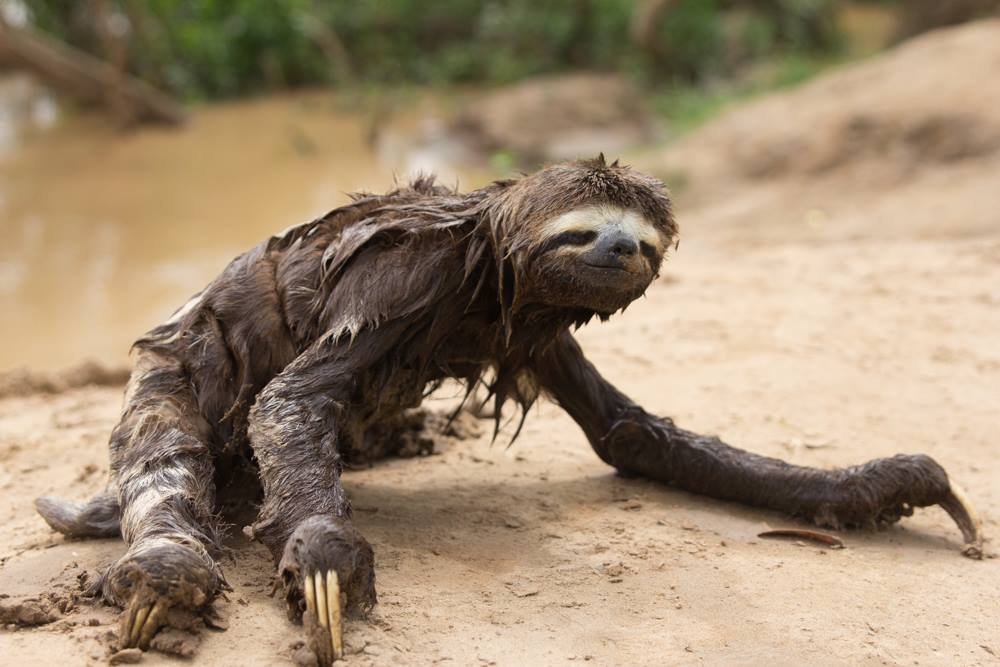
\includegraphics[scale=0.35]{pictures/mokry_leniwiec.jpg}
        \caption{Mokry leniwiec}
        \label{fig:sloth}
    \end{figure}
\end{document}
